\chapter{Theoretical Background and Related Work}
\label{chapter:background} 

In chapter \ref{chapter:intro} a brief general analysis of stereo geometry and methods has been provided. 
In this chapter a more precise revision of the theoretical tools that stereo matching methods exploit is presented.
Epipolar geometry, camera calibration and disparity estimation algorithms are specifically described. 
Starting from the necessary mathematical basis, the discussion moves on the disparity estimation algorithms. 
Then, the chapter focus on the main benefits and drawbacks of standard and novel approaches in depths computation.
Comparison between stereo-geometry based and deep learning based algorithms is proposed, to provide a clear explanation of the decisions implemented. 

\section{Epipolar geometry and Rectifiation}
\label{sec:eipolarandrect}

Fundamental problem of stereo vision is the estimation of 3D locations of points from at least two corresponding input images.
This process, which comprises concurrent computation of both 3D geometry and camera pose, is generally known as structure from motion \cite{Szeliski2011}.\\
In the explanation of these topics it is necessary to start discussing about the triangulation.
Then, the concept of epipolar geometry is outlined and after that the notions of camera calibration and rectification. 

\subsection{Triangulation}
\label{subsec:triangulation}

\begin{figure}[t]
	\begin{center}
		{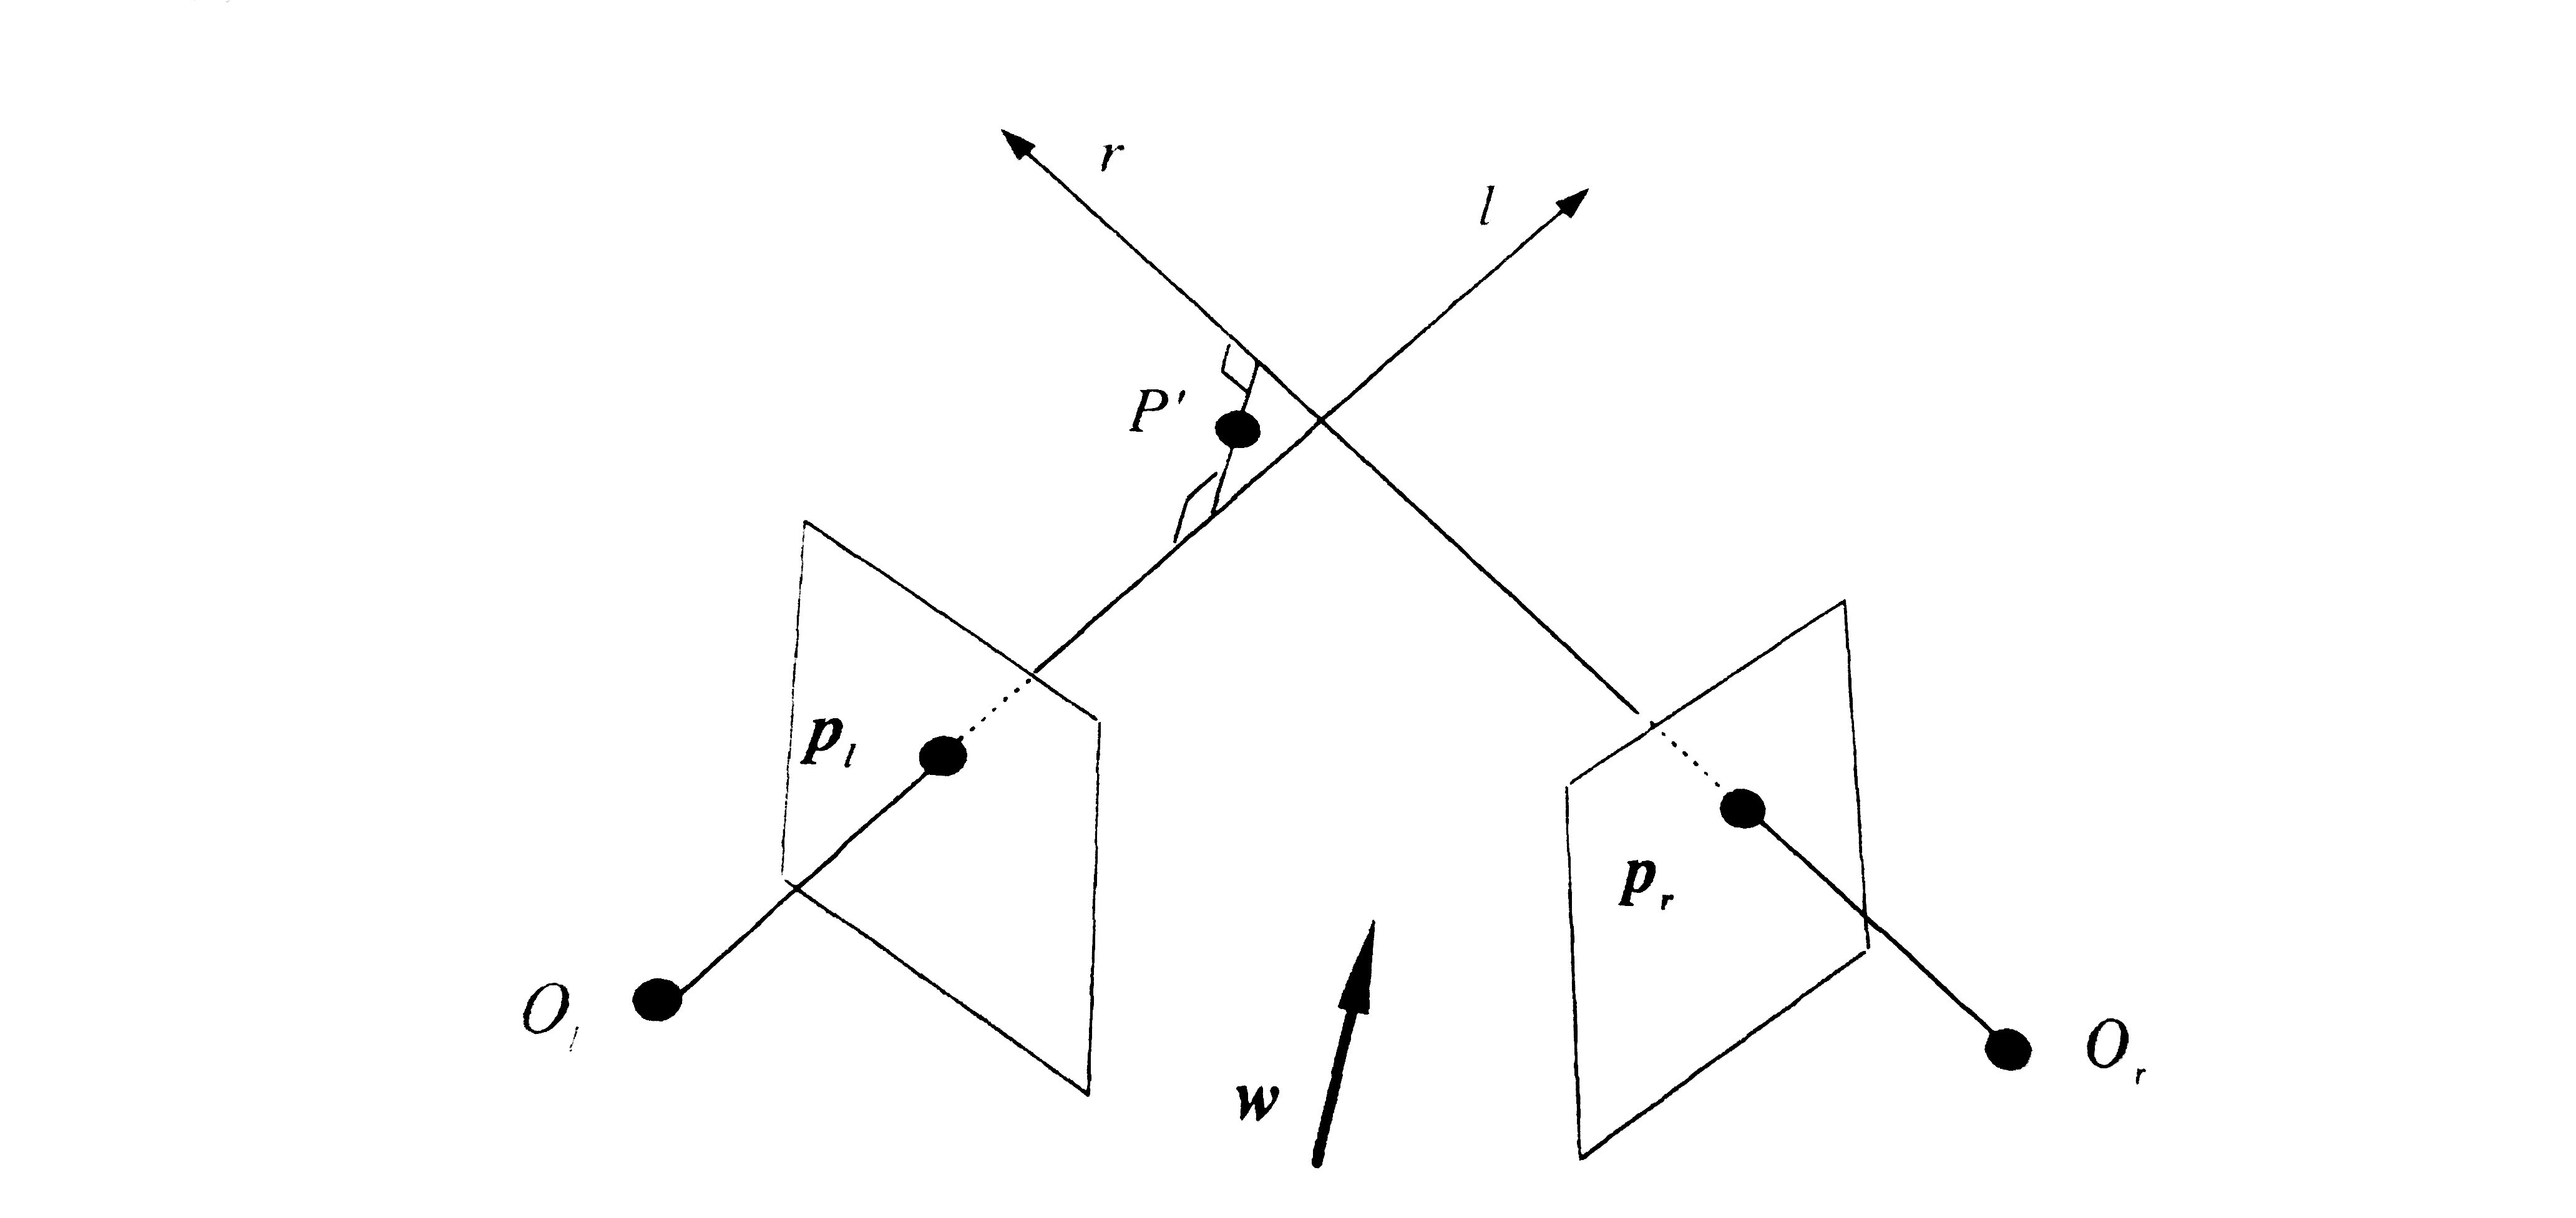
\includegraphics[width=.8\textwidth]{images/triangulation}}
\caption{3D triangulation by finding point $P'$ that lies nearest to all of the optical rays}
\label{fig:triangulation}
	\end{center}
\end{figure}

Triangulation is the problem of detecting 3D points positions from a collection of corresponding 2D image locations, assuming that camera positions are known.
Figure \ref{fig:triangulation} shows one of the easiest methods to tackle this problem. 
Objective is to evaluate the 3D position of $P'$ that have the smallest error to all of the 3D optical rays coming from the camera centers, which identify the 2D point locations in the image plane, i.e. $P_r$ and $P_l$.
As shown in Figure \ref{fig:triangulation}, the rays starts from the camera centers, $O_j$ and go in direction of $r$ and $l$, which can be defined using the camera matrix $ \{ P_j = K_j [ R_j | t_j ] \} $.
The closest point to $P$ on this ray minimizes the distance
\begin{equation}\label{eqn:mindist}
	\Vert O_j + d_j \hat{v}_j - P \Vert^2
\end{equation}
Therefore, because of the minimum is $d_j = \hat{v}_j \cdot (p - c_j)$, the nearest points are calculated as:
\begin{equation}\label{eqn:closestpoint}
	q_j = O_j + (\hat{v}_j \hat{v}_j^\top)(P - O_j) = O_j + (P - O_j)_{\Vert}
\end{equation}
Hence, the optimal value for $P$, obtained solving a least square problem, becomes,
\begin{equation}\label{eqn:solP}
	P = \Big[ \sum_j (I - \hat{v}_j \hat{v}_j^\top ) \Big]^{-1} = \Big[ \sum_j (I - \hat{v}_j \hat{v}_j^\top )O_j \Big]
\end{equation}

\subsection{Epipolar geometry}
\label{subsec:epipolargeom}

\begin{figure}[t]
	\begin{center}
		{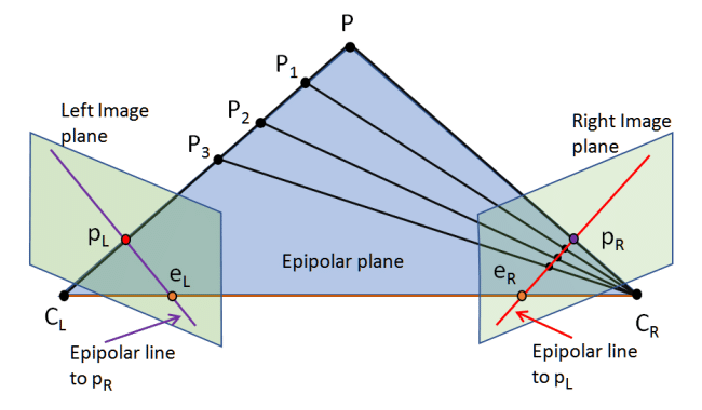
\includegraphics[width=.8\textwidth]{images/epipolar-geometry-2}}
\caption{Epipolar geometry. Image point $m$ back-projects to a ray in a 3D space defined by $C$ and $m$. This ray becomes a line $l'$ in the second view. The image of $X$ must lie on $l'$}
\label{fig:epipolargeom-2}
	\end{center}
\end{figure}

The intrinsic projective geometry between two views is known as epipolar geometry.
It is only dependent on the cameras' internal parameters and pose.
The $3 \times 3$ rank 2 matrix that defines this geometry is the fundamental matrix $F$.\\
The epipolar geometry is the basis for finding corresponding points in stereo matching. 
It is basically defined by the intersection between image planes and the one on which the cameras baseline lies.\\
A fundamental property, that makes this geometry extremely useful, is that image points, space point and camera centers are coplanar. 
Assuming that only $m_l$ is known, that geometry allows to constraint the corresponding point $m_r$. 
The epipolar plane is defined by the baseline and the ray that comes from $m_l$. 
Hence, knowing that $m_r$ lies on the same plane, that point belongs to $l_r$, i.e. the intersection between the epipolar and the second image plane. 
Therefore, exploiting this property, the searching of corresponding points is constrained to only one line inside the image.\\
Mathematical definition of the epipolar geometry is the fundamental matrix $F$.
As already demonstrated through Figure \ref{fig:epipolargeom-2}, for each point $p_L$ in one image, the corresponding epipolar line $e_R$ to that point belongs to the other image plane. 
Moreover, any point $p_R$ in the second image, which is related to point $p_L$, lies on $e_R$.
Hence, the epipolar line is described as the projection in the second image of the ray that comes from the point in the first image, passing through its camera center.
This defines a map, $p_L \rightarrow e_R$, which relates the points in one image with the corresponding epipolar lines in the second image.
This correlation, between points and lines, is represented by the fundamental matrix $F$.\\
Considering the aforementioned map $p_L \rightarrow e_R$ described by $F$, an important property of the fundamental matrix is defined,
\begin{equation}\label{eqn:fundmatprop}
	p_R^\top F p_L = 0
\end{equation}
Therefore, assuming two corresponding points $P_L$ and $p_R$, it is known that $p_R$ lies on the epipolar line $l_R = F p_L$. 
Thus, the mathematical correlation is,
\begin{equation}
	0 = p_R^\top e_R = p_R^\top F p_L
\end{equation}
Reciprocally, if image points comply the relation \ref{eqn:fundmatprop}, then the rays identified by these points are coplanar. 
For point corresponding this is a necessary condition.
Equation \ref{eqn:fundmatprop} is extremely important because it allows to characterize the fundamental matrix without reference to the camera matrices \cite{hartley2004multiple}.
Thus, using at least 7 correspondences, it is possible to recover the fundamental matrix $F$. 
This estimation is known as \textit{weak calibration}.\\
\textbf{Maybe add 8-point algorithm description}

\subsection{Rectification}
\label{subsec:rectification}

Image rectification is defined as the process of obtaining a pair of \textit{matched epipolar projections} from a pair of stereo images, which are taken from generally differing viewpoints.
In the rectified projections the epipolar lines become parallel with respect to the x-axis. 
Thus, they match between the stereo pair and so the disparities are in the x-direction only.\\
In order to obtain a rectified stereo pair, 2D projective transformations are employed to the images, so that the epipolar lines can match.
Using this method, the transformations are built up in a way that the corresponding points have almost the same x-coordinate.
Actually, this strategy leads to a minimal distortion on the images, being the two transformations arbitrary. 
However, working on rectified images, the matching problem is highly simplified, being correlated only to epipolar geometry and near-correspondence. \\
Core problem of this section is to find the appropriate projective transformation $H$. 
Indeed, to get epipolar lines parallel with x-axis, the epipole should be mapped to an infinite point. 
This, has to be done correctly, otherwise intensive projective distortion of the image can happen.
For this reason, constraints are put on the definition of $H$.\\
First of all, restricting $H$ to be a rigid transformation in the neighbourhood of a given point\footnote{this means that to first-order, the neighbourhood of the point may be subjected to rotation and translation only}, the errors are reduced.\\
Once the epipole has been mapped to infinity, it is then necessary define a map to match the corresponding epipolar lines.
This resampling is build up in such a way that, being $e_L$ and $e_R$ any pair of epipolar lines, then,
\begin{equation}
	H^{-\top} e_L = H'^{-\top} e_R
\end{equation}
Satisfying the condition above, a matched pair of transformations is recovered.\\
Specifically, at first $H'$ is chosen, so that it can map the epipole $e_R$ to infinity. 
Then the matching transformation $H$ is defined minimizing the sum-of-square distances,
\begin{equation}\label{eqn:matchtransfconstr}
	\sum_i d(H p_{L_i}, H'p_{R_i})^2
\end{equation}

Therefore, the full algorithm can be summarized as follows.\\
The outcome of this resampling process is a pair of stereo images whose epipolar lines are horizontal.
Hence, the disparities are calculated along the epipolar lines. 
First of all, at least seven corresponding matches are defined.
This allows to compute the fundamental matrix $F$, applying the so called eight-point algorithm, and after that the two epipoles are found.
After that, there is the selection of the projective transformation $H'$, that maps the epipole of the support image to infinity.
The corresponding transformation $H$ is found solving the least-square problem.
Finally both of the input images are resampled according to $H$ and $H'$.

\section{Stereo methods and dense correspondence}
\label{sec:stereometh}

\textbf{Take the part already written in the introduction}\\
\textbf{Refactoring needed between the 2 chapters}

\subsection{Stereo geometry based methods}

\subsection{Deep learning based methods}
\label{subsec:deeplearnmeth}



\subsection{Referring to sources}

\emph{Haapasalo~\cite{HaapasaloThesis} researched database algorithms
  that allows use of previous versions of the content stored in the
  database.} This kind of marking means that this paragraph (or until
the next reference is given) is based on the source mentioned in the
beginning.  Giving the source you should use only the family name of
the first author of the article, and not give any hints about what is
the type of the article that is referred nor its title.

\emph{B+-trees offers one way to index data that is stored in to a
  database. Multiversion B+-trees (MVBT) offer also a way to restore
  the data from previous versions of the database. Concurrent MVBT
  allows many simultaneous updates to the database that is was not
  possible with MVBT.~\cite{HaapasaloThesis}} When the marking is
after the period, the reference is retrospective: all the paragraph
(or after previous reference marking) is based on the source given in
its end. If the content is very broad, you can start with saying
\emph{According to Haapasalo}, then continue referring the source with
several separate sentences, and in the end put the marking of your
source \emph{ that shows that CMVBT are the
  best. ~\cite{HaapasaloThesis}}. 

If your paragraph has several sources, the above mentioned styles are
not proper. The reader of your thesis cannot know which of your
sources give which of the statements. In this case, it is better to
use more finegraded refering where the reference markings that are
embedded in the sentences. For example, \emph{the multiversion B+-tree
  (MVBT) index of Becker et al.~\cite{becker:1996:mvbt} allows database
  users to query old versions of the database, but the index is not
  transactional.
  It's successor, the transactional MBVT (TMVBT), allows a single transaction
  running in its own thread or process to update the database concurrently
  with other transactions that only read the
  database~\cite{haapasalo:2009:tmvbt}. 
  Further development, titled the concurrent MBVT (CMVBT),
  allows several transactions to perform updates to the database at the same
  time~\cite{HaapasaloThesis}}. 
  Here, the references are marked before
  the period in the sentences where they are used. You should never
  but all these sources in the end of the paragraph. Referring several
  source at once should only used when you give a set of examples.

Finally, direct quotes are allowed. However, often you should avoid
them since they do not usually fit in to your text very well. Using
direct quotes has two tricks: quotation marks and the source.  \emph{
  ``Even though deletions in a multiversion index must not physically
  delete the history of the data items, queries and range scans can
  become more efficient, if the leaf pages of the index structure are
  merged to retain optimality.''~\cite{HaapasaloThesis}} Quotes are
hard to make neatly since you should use only as much as needed
without changing the text. Moreover, you often do not really
understand what the author has mentioned with his wordings if you
cannot write the same with your own words. Remember also that never
cut and paste anything without marking the quotation marks right away,
and in general, never cut and paste anything at all!

Sometimes getting the original source can be almost impossible. In an
extremely desperate situation, you can refer with structure \emph{ms
  X~[\ldots] according to mr Y~[\ldots] defined that}, if you find a
source that refers to the original source. Note also that the
reference marking is never used as sentence element (example of how 
\textbf{not} to do it: \emph{\cite{HaapasaloThesis} describes
an optimal algorithm for indexing multiversiond databases.}).



